% ============================================================================
% DevBridge -- B.Tech Project Progress Report
% Overall architecture, M5 (CV Verification Engine) pipeline and progress,
% M6 (Skill Graph) architecture, scoring model and progress.
%
% Compile with pdflatex (two passes) or tectonic. Uses only packages shipping
% in any standard TeX Live / MiKTeX install.
% ============================================================================
\documentclass[11pt,a4paper]{article}

\usepackage[T1]{fontenc}
\usepackage[utf8]{inputenc}
\usepackage{mathpazo}
\usepackage[scaled=0.92]{helvet}
\usepackage{microtype}

\usepackage[a4paper,margin=2.1cm,headheight=14pt]{geometry}
\usepackage{fancyhdr}
\usepackage{titlesec}
\usepackage{enumitem}
\setlist[itemize]{leftmargin=1.2em, itemsep=1pt, topsep=2pt}
\setlist[enumerate]{leftmargin=1.4em, itemsep=1pt, topsep=2pt}

\usepackage{amsmath,amssymb}
\usepackage{array}
\usepackage{booktabs}
\usepackage{longtable}
\usepackage{float}
\usepackage[table]{xcolor}
\usepackage{graphicx}
\usepackage{tikz}
\usetikzlibrary{arrows.meta,positioning,calc}
\usepackage{framed}
\usepackage[colorlinks=true,linkcolor=accentlink,citecolor=accentlink,
            urlcolor=accentlink,pdfborder={0 0 0}]{hyperref}

% Long, space-free identifiers appear in running text; raise TeX's tolerance
% for a loose line and give it a stretch reserve rather than letting a rare
% token overflow the margin.
\tolerance=9999
\emergencystretch=3em
\hbadness=10000

\definecolor{accent}{HTML}{1C6A5E}
\definecolor{accent2}{HTML}{2E8C7C}
\definecolor{accentlink}{HTML}{15544A}
\definecolor{negative}{HTML}{9C4A21}
\definecolor{warn}{HTML}{8A6A17}
\definecolor{m5color}{HTML}{6244C5}
\definecolor{inkgray}{HTML}{3E4A46}
\definecolor{mutedgray}{HTML}{6B7772}
\definecolor{rulegray}{HTML}{C2CEC8}
\definecolor{sunken}{HTML}{EBF0ED}
\colorlet{shadecolor}{sunken}

\DeclareMathOperator{\logit}{logit}
\DeclareMathOperator{\sig}{sigmoid}

\titleformat{\section}
  {\normalfont\sffamily\Large\bfseries\color{accent}}
  {\thesection}{0.6em}{}[{\color{rulegray}\titlerule[1pt]}]
\titleformat{\subsection}
  {\normalfont\sffamily\large\bfseries\color{inkgray}}
  {\thesubsection}{0.5em}{}
\titleformat{\subsubsection}
  {\normalfont\sffamily\bfseries\color{inkgray}}
  {\thesubsubsection}{0.5em}{}
\titlespacing*{\section}{0pt}{1.1em}{0.6em}
\titlespacing*{\subsection}{0pt}{0.9em}{0.35em}
\titlespacing*{\subsubsection}{0pt}{0.7em}{0.2em}

\pagestyle{fancy}
\fancyhf{}
\renewcommand{\headrulewidth}{0.4pt}
\fancyhead[L]{\small\sffamily\color{mutedgray}DevBridge -- Progress Report}
\fancyhead[R]{\small\sffamily\color{mutedgray}\today}
\fancyfoot[C]{\small\sffamily\color{mutedgray}\thepage}

\newenvironment{notebox}[1]{%
  \def\FrameCommand{{\color{warn}\vrule width 2.2pt}\hspace{8pt}}%
  \MakeFramed{\advance\hsize-\width \FrameRestore}%
  \noindent{\sffamily\footnotesize\bfseries\color{warn}#1}\par\smallskip
  \small
}{%
  \par\endMakeFramed
}

\newcolumntype{L}[1]{>{\raggedright\arraybackslash}p{#1}}
\newcolumntype{C}[1]{>{\centering\arraybackslash}p{#1}}

% ============================================================================
\begin{document}
\thispagestyle{empty}

\begin{center}
{\sffamily\footnotesize\bfseries\color{mutedgray}\MakeUppercase{B.Tech Project -- Progress Report}}\\[0.55cm]
{\sffamily\Huge\bfseries\color{accent} DevBridge}\\[0.2cm]
{\sffamily\large\color{inkgray} A Verified-Talent Freelance Platform}\\[0.55cm]

\begin{tikzpicture}\draw[accent, line width=1pt] (0,0) -- (7,0);\end{tikzpicture}\\[0.5cm]
\begin{tabular}{ll}
\sffamily\bfseries\color{mutedgray} Submitted by & \emph{[Name --- fill in name / roll number]} \\[2pt]
\sffamily\bfseries\color{mutedgray} Modules covered & M5 (CV Verification Engine) \ $\cdot$ \ M6 (Skill Graph) \\[2pt]
\sffamily\bfseries\color{mutedgray} Date & \today \\
\end{tabular}
\end{center}
\vspace{0.3cm}
\noindent\small\color{inkgray}
This report summarises the overall system architecture agreed for DevBridge, the
progress made on Module 5 (CV Verification Engine), and the progress made on
Module 6 (Skill Graph) -- the module this report's author owns.
\normalsize\color{black}
\vspace{0.2cm}

% ============================================================================
\section{System Architecture and Design Rationale}
% ============================================================================

\subsection{The Technical Thesis}

DevBridge is a platform for verifying developer competence from evidence
rather than self-report. Its central technical claim is:

\begin{notebox}{Central claim}
Developer competence can be estimated from heterogeneous, partially reliable
behavioural evidence -- commit history, contest performance, delivery
outcomes, CV claims -- by fusing it into a single calibrated
\textbf{per-skill latent-ability estimate with explicit uncertainty that
grows over time}. The fused estimate is more reliable than any single
evidence stream, and its stated confidence is empirically accurate.
\end{notebox}

Everything else in the platform -- the marketplace, escrow, the recruiter
console -- is supporting infrastructure. It is competently engineered, but it
is the skill-graph model and the verification pipeline that constitute the
project's technical contribution.

\subsection{Architectural Principles}

Six rules, agreed before any module's implementation began, from which every
later design decision follows.

\begin{center}\small
\begin{tabular}{@{}L{3.1cm}L{10.6cm}@{}}
\toprule
\textbf{Principle} & \textbf{What it means in practice} \\
\midrule
Contracts before code & Every module publishes a schema/OpenAPI contract before implementation starts. A module is ``done'' when it satisfies its contract tests. \\
No shared database & Every module owns its storage exclusively. Cross-module communication happens over HTTP or events, never a shared table. \\
Evidence is append-only & Nothing overwrites a record. Every score is \emph{derived and recomputable} from the event log at any point in time. \\
The LLM boundary & A language model may translate unstructured text into structured data, or structured findings into prose. It may \textbf{never} produce a number that enters a score, and never decide whether a claim is true. \\
No trained models & Every quantitative judgement comes from descriptive statistics against a reference distribution or a closed-form update rule -- never a fitted classifier. There is no labelled training set anywhere in the pipeline. \\
Confidence, never verdicts & Every module emits a value with confidence and evidence references. No module emits a boolean pass/fail or a hiring recommendation. \\
\bottomrule
\end{tabular}
\end{center}

\subsection{Module Map}

The platform is organised into fifteen independently deployable modules
across five layers. M5 and M6 -- the subjects of this report -- are
highlighted.

\begin{center}\small
\begin{tabular}{@{}lL{2.6cm}L{9.4cm}@{}}
\toprule
\textbf{Layer} & \textbf{Module} & \textbf{Responsibility} \\
\midrule
\textit{0 -- Substrate} & M0 core-gateway & Edge routing, authentication, rate limiting \\
 & M1 identity-consent & Accounts and an append-only consent ledger \\
 & M2 evidence-bus & Event backbone and schema registry \\
\midrule
\textit{1 -- Evidence producers} & M3 code-provenance & Authorship and originality verification from repository history \\
 & M4 assessment-engine & Sandboxed technical assessments \\
 & \cellcolor{sunken}\textbf{M5 cv-verification} & \cellcolor{sunken}\textbf{The standalone CV verification engine -- \S2} \\
\midrule
\textit{2 -- The graph} & \cellcolor{sunken}\textbf{M6 skill-graph} & \cellcolor{sunken}\textbf{Fuses all evidence into calibrated per-skill ability -- \S3} \\
\midrule
\textit{3 -- Marketplace} & M7 marketplace & Postings, matching, contract state machine \\
 & M8 delivery-review & Post-gig review; feeds evidence back to M6 \\
 & M9 payments-escrow & Escrow ledger and payout \\
 & M10 financing & Advance-rate decisioning, priced off the skill graph \\
\midrule
\textit{4 -- Enterprise} & M11 enterprise-api & Public verification API, metering \\
 & M12 ats-connector & ATS integration adapters \\
 & M13 recruiter-console & Consent-gated search over the verified pool \\
\midrule
\textit{Cross-cutting} & M14 eval-harness & Datasets, metrics, ablation, calibration \\
 & M15 web-clients & Front-ends against the public contracts only \\
\bottomrule
\end{tabular}
\end{center}

\subsection{Block Diagram}

Evidence flows one way, bottom to top: producer modules generate typed
evidence, the skill graph fuses it into calibrated ability, and the
marketplace and enterprise layers read from that fused state. No module
reads another's private database.

\begin{figure}[H]
\centering
% MERMAID PLACEHOLDER -- render figures/block-diagram.mmd (source below/
% separately provided) to figures/block-diagram.pdf (preferred) or .png,
% drop the file next to this .tex file at that relative path, and this
% \includegraphics line will pick it up unchanged.
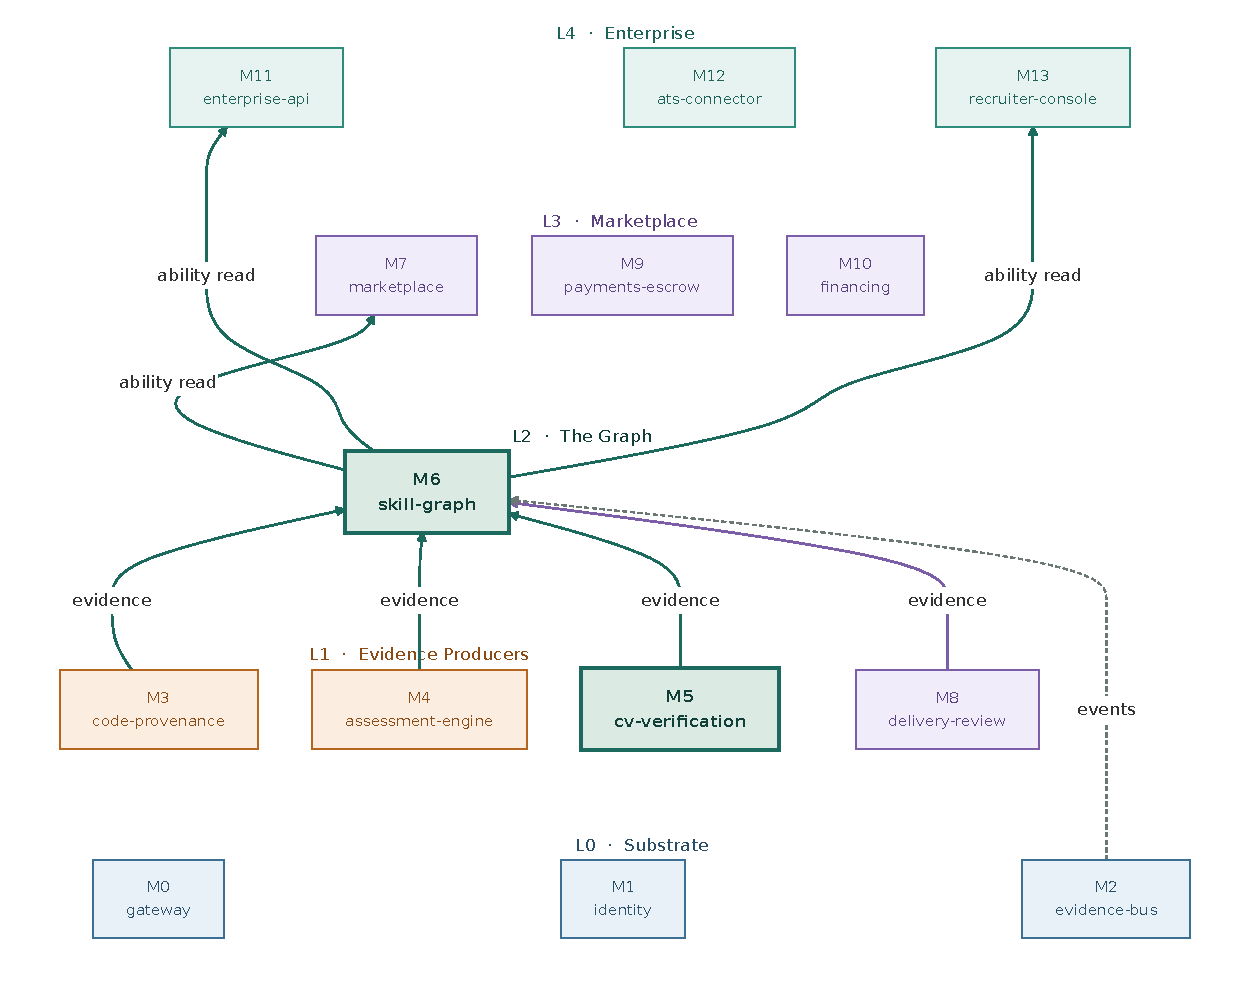
\includegraphics[width=\textwidth]{figures/block-diagram.pdf}
\caption{DevBridge module map. M5 and M6 are shaded. Arrows show the
direction evidence and ability estimates flow; no module reads another's
private storage.}
\end{figure}

\subsection{Where Language Models Are Used, and Where They Are Not}

A model is used only where no deterministic alternative exists: extracting
structured claims from free-text CVs (M5), generating novel assessment
challenges (M4), and rendering computed findings into prose (M5, M6-adjacent
reporting). A model is explicitly \textbf{forbidden} from computing any
score, judging authorship, deciding timeline consistency, or issuing any
verdict -- those are deterministic rule engines, statistical distance
measures, or closed-form filters, precisely so that every number in the
system can be recomputed and audited without re-running a model.

% ============================================================================
\section{Module 5 --- CV Verification Engine}
% ============================================================================

\subsection{Purpose and Constraints}

M5 turns an uploaded CV into a structured report of what the evidence
supports, what it contradicts, and what could not be checked. It is built as
a \textbf{standalone product}: it runs on any CV, including one from a person
with no DevBridge account; it imports nothing from the rest of the platform;
and it emits findings, never a verdict. There is no overall trust score, no
threshold, and no pass/fail -- a design constraint enforced in code, not only
stated in documentation.

\subsection{The Pipeline}

The pipeline runs in nine steps. Steps~2, 3 and 9 call a language model;
every other step is deterministic code with no network dependency beyond the
evidence lookups in step~6.

\begin{figure}[H]
\centering
\resizebox{\textwidth}{!}{%
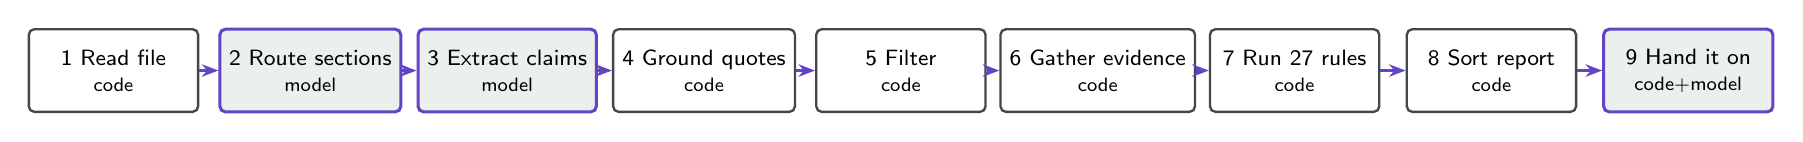
\begin{tikzpicture}[
  stepbox/.style={draw=inkgray, line width=0.85pt, rounded corners=2pt, fill=white,
               font=\sffamily\footnotesize, minimum height=1.05cm, minimum width=2.15cm, align=center},
  model/.style={draw=m5color, line width=1.1pt, rounded corners=2pt, fill=sunken,
                font=\sffamily\footnotesize, minimum height=1.05cm, minimum width=2.15cm, align=center},
  arr/.style={-{Stealth[length=6pt]}, line width=0.9pt, m5color},
]
  \node[stepbox]  (s1) at (0,0)    {1 Read file\\\scriptsize code};
  \node[model] (s2) at (2.5,0)  {2 Route sections\\\scriptsize model};
  \node[model] (s3) at (5.0,0)  {3 Extract claims\\\scriptsize model};
  \node[stepbox]  (s4) at (7.5,0)  {4 Ground quotes\\\scriptsize code};
  \node[stepbox]  (s5) at (10.0,0) {5 Filter\\\scriptsize code};
  \node[stepbox]  (s6) at (12.5,0) {6 Gather evidence\\\scriptsize code};
  \node[stepbox]  (s7) at (15.0,0) {7 Run 27 rules\\\scriptsize code};
  \node[stepbox]  (s8) at (17.5,0) {8 Sort report\\\scriptsize code};
  \node[model] (s9) at (20.0,0) {9 Hand it on\\\scriptsize code+model};

  \foreach \a/\b in {s1/s2,s2/s3,s3/s4,s4/s5,s5/s6,s6/s7,s7/s8,s8/s9}
    \draw[arr] (\a) -- (\b);
\end{tikzpicture}%
}
\caption{The nine-step verification pipeline. A quote that cannot be found
in the source document is dropped at step~4; a real but unusable claim is
refused at step~5; every rule outcome at step~7 is one of
\texttt{discrepancy}, \texttt{corroborated}, \texttt{abstain} or
\texttt{clean} -- never a verdict.}
\end{figure}

\begin{center}\small
\begin{tabular}{@{}L{2.1cm}L{11.0cm}@{}}
\toprule
\textbf{Step} & \textbf{What happens} \\
\midrule
1 Read file & PDF/DOCX/OCR extraction to normalised text with page offsets. \\
2--3 Extract & The model proposes claims (employment, education, skills, projects, achievements) with a verbatim quoted span -- no character positions are trusted from the model. \\
4 Ground & Every quoted span must literally exist in the source document (exact or a fuzzy match $\geq 0.92$); a claim that fails is dropped and counted. \\
5 Filter & A real but unusable claim (value not supported by its own sentence, duplicate, excluded exam) is refused. \\
6 Gather evidence & GitHub, Codeforces, LeetCode and live-URL lookups, only for accounts the CV itself names. A failed lookup becomes a typed gap, never a guess. \\
7 Run the checks & 27 pure-function rules, each producing a \texttt{discrepancy}, an \texttt{abstain} with a reason, a \texttt{corroborated}, or a \texttt{clean}. \\
8 Sort & Findings sort into five buckets by the rule's own tier -- \emph{Contradicted}, \emph{Needs context}, \emph{Verified}, \emph{Not evaluated}, \emph{Out of scope} -- never into a single score. \\
9 Hand it on & The same report as JSON/API, a one-sentence-per-finding narrative, a reviewer worksheet, and (with consent) skill signals to M6. \\
\bottomrule
\end{tabular}
\end{center}

\subsection{Progress to Date}

\begin{center}\small
\begin{tabular}{@{}L{3.4cm}L{3.2cm}L{6.0cm}@{}}
\toprule
\textbf{Metric} & \textbf{Value} & \textbf{Note} \\
\midrule
Checks built & 28 / 34 reachable & 6 remaining need issuer APIs DevBridge does not yet have \\
Automated tests & 474 passing, 0 failing & plus 5/5 on the live-model integration suite \\
Static analysis & clean & \texttt{ruff} and \texttt{mypy --strict} across the codebase \\
Source size & $\sim$9{,}960 lines & across the pipeline, rule engine and API \\
Documents evaluated & 3 real CVs & student, synthetic, and professional profiles \\
Injected-error detection & 15/15, 7/7, 2/2 & 0 false positives across all three documents \\
Span-grounding failures & 0 & every dropped claim was refused text, never fabricated \\
\bottomrule
\end{tabular}
\end{center}

\begin{center}\small
\begin{tabular}{@{}L{2.6cm}C{1.3cm}L{4.1cm}L{4.6cm}@{}}
\toprule
\textbf{Check family} & \textbf{Built} & \textbf{Basis} & \textbf{Status of the rest} \\
\midrule
Document-intrinsic & 11 / 11 & the CV alone (timeline, tenure, dates) & complete \\
GitHub & 10 / 10 & the account and repositories named & complete \\
Contest platforms & 5 / 6 & Codeforces, LeetCode & CodeChef has no public API \\
Deployments & 1 / 2 & does the linked site respond & ``matches description'' needs a reviewer \\
Credentials & 1 / 5 & narrative rendering only & no issuer APIs available yet \\
Human-judgement & 0 / 6 & \emph{by design} & prepared as a worksheet, never automated \\
\bottomrule
\end{tabular}
\end{center}

The pipeline is feature-complete for everything currently reachable without
an issuer integration. The two items of remaining work are a larger
hand-labelled evaluation corpus (to measure extraction precision/recall
directly, alongside the detection-rate figures above) and issuer-API
integrations for the credential family.

% ============================================================================
\section{Module 6 --- Skill Graph}
% ============================================================================

\subsection{Purpose}

M6 takes verified evidence about a developer -- from M5, M3, M4 and delivery
history -- and maintains a calibrated belief about that developer's ability
in each individual skill: not a rating, but a Gaussian estimate that narrows
as evidence arrives and widens again as it ages. There is no overall score;
every answer is per skill, with an explicit interval.

\subsection{Module Architecture}

Six submodules, evidence flowing one way. The ontology is consulted, never
written to, by three of the six; the integrity layer reads the finished
graph and writes nothing back into it.

\begin{figure}[H]
\centering
\resizebox{\textwidth}{!}{%
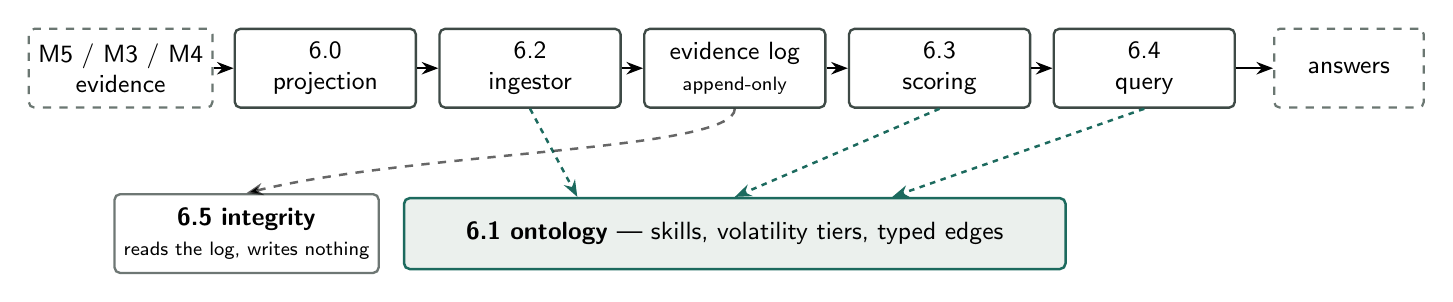
\begin{tikzpicture}[
  box/.style={draw=inkgray, line width=0.85pt, rounded corners=2pt, fill=white,
              font=\sffamily\small, minimum height=1.0cm, minimum width=2.3cm, align=center},
  endpt/.style={draw=mutedgray, line width=0.8pt, dashed, rounded corners=2pt, fill=white,
                font=\sffamily\small, minimum height=1.0cm, minimum width=1.9cm, align=center},
  onto/.style={draw=accent, line width=0.9pt, rounded corners=2pt, fill=sunken,
               font=\sffamily\small, minimum height=0.9cm, align=center},
  arr/.style={-{Stealth[length=6pt]}, line width=0.9pt},
  dotted/.style={-{Stealth[length=6pt]}, line width=0.9pt, accent, dash pattern=on 2pt off 2pt},
]
  \node[endpt] (in)   at (0,0)    {M5 / M3 / M4\\evidence};
  \node[box]   (p0)   at (2.6,0)  {6.0\\projection};
  \node[box]   (p2)   at (5.2,0)  {6.2\\ingestor};
  \node[box]   (log)  at (7.8,0)  {evidence log\\\scriptsize append-only};
  \node[box]   (p3)   at (10.4,0) {6.3\\scoring};
  \node[box]   (p4)   at (13.0,0) {6.4\\query};
  \node[endpt] (out)  at (15.6,0) {answers};

  \foreach \a/\b in {in/p0,p0/p2,p2/log,log/p3,p3/p4,p4/out}
    \draw[arr] (\a) -- (\b);

  \node[onto, minimum width=8.4cm] (onto) at (7.8,-2.1)
       {\textbf{6.1 ontology} --- skills, volatility tiers, typed edges};
  \draw[dotted] (p2.south) -- ([xshift=-2.0cm]onto.north);
  \draw[dotted] (p3.south) -- (onto.north);
  \draw[dotted] (p4.south) -- ([xshift=2.0cm]onto.north);

  \node[box, draw opacity=.75, minimum width=3.0cm] (integ) at (1.6,-2.1)
       {\textbf{6.5 integrity}\\\scriptsize reads the log, writes nothing};
  \draw[arr, dashed, draw opacity=.6] (log.south) .. controls (7.8,-1.05) and (3.8,-1.05) .. (integ.north);
\end{tikzpicture}%
}
\caption{The six M6 submodules. 6.1 exposes three read-only questions
(\texttt{knows()}, \texttt{tier()}, \texttt{relations()}); nothing downstream
writes back to it. 6.5 changes no score it reads.}
\end{figure}

\subsection{The Scoring Model}

Each (developer, skill) pair is a Gaussian belief in \textbf{logit space}:
$x = \logit(\theta)$, unbounded, so the Kalman update below is exact rather
than an approximation later clipped to $[0,1]$.

\paragraph{Observation.} Every event yields an observed value and a
variance:
\[
\sigma^2_{\mathrm{obs}} = \frac{S_0}{\text{reliability} \times \text{relevance} \times \text{strength}},
\qquad S_0 = 0.10.
\]
Relevance sits in the variance, never the observed value -- a signal that is
only partially about a skill is treated as \emph{less certain}, not as
\emph{weaker evidence of a lower ability}.

\paragraph{Update.} A closed-form Kalman step, no fitting:
\[
K = \frac{\sigma^2}{\sigma^2+\sigma^2_{\mathrm{obs}}}, \qquad
\mu' = \mu + K(\logit(\text{observed})-\mu), \qquad
\sigma^{2\prime} = \sigma^2(1-K).
\]

\paragraph{Decay.} Between observations, uncertainty grows and the mean
reverts toward the prior:
\[
\sigma^2(t) = \sigma^2(\tau) + \lambda_s\,\Delta t, \qquad
\mu(t) = \mu + (\mu_0-\mu)\big(1-e^{-\Delta t\,\lambda_s/k}\big).
\]
$\lambda_s$ depends on the skill's volatility tier (fundamental, ecosystem,
framework) -- a framework goes stale in about 1.3 years, a fundamental in
about 9.6.

\paragraph{Display.} The published number is a \textbf{lower confidence
bound}, not the mean:
\[
\text{score} = \sig(\mu - z\sigma), \qquad z = 1.0.
\]
Thin evidence and abundant evidence can share a mean; only the second
produces a high published score, because only its interval has closed up.

\subsection{Worked Example}

The table below is a real trace from the shipped scoring engine for one
developer's \texttt{go} skill: a repository commit, a corroborated CV claim,
and 81 days of subsequent silence.

\begin{center}\small
\begin{tabular}{@{}L{3.6cm}rrrr@{}}
\toprule
\textbf{Step} & $\mu$ & $\sigma$ & \textbf{score} & \textbf{mean} \\
\midrule
prior (no evidence) & $-1.099$ & 1.300 & 0.083 & 0.250 \\
+ repository commit (168 commits) & $+0.436$ & 0.467 & 0.492 & 0.607 \\
+ corroborated CV claim & $+0.611$ & 0.313 & 0.574 & 0.648 \\
81 days later, published & $+0.496$ & 0.350 & \textbf{0.536} & 0.622 \\
\bottomrule
\end{tabular}
\end{center}

The published score rises from 0.083 to 0.574 mainly because the
\emph{interval closes} (width $0.47\to0.14$), not because the mean moves
furthest. It then falls to 0.536 purely from elapsed time -- the system
stating it knows less, never that the developer regressed.

\subsection{Progress to Date}

Seven packages, all independently tested.

\begin{center}\small
\begin{tabular}{@{}llrr@{}}
\toprule
\textbf{Sub\-module} & \textbf{Package} & \textbf{Lines} & \textbf{Tests} \\
\midrule
Facade & \texttt{m6} & 316 & 37 \\
6.1 ontology & \texttt{m6\_ontology} & 411 & 77 \\
6.0 projection & \texttt{m6\_projection} & 904 & 108 \\
6.2 ingestor & \texttt{m6\_ingestor} & 711 & 76 \\
6.3 scoring & \texttt{m6\_scoring} & 1{,}019 & 129 \\
6.4 query & \texttt{m6\_query} & 618 & 97 \\
6.5 integrity & \texttt{m6\_integrity} & 412 & 38 \\
\midrule
\textbf{Total} & & \textbf{4{,}391} & \textbf{562} \\
\bottomrule
\end{tabular}
\end{center}

\textbf{Validation.} A parameter-recovery experiment -- 300 synthetic
developers of known ability, 12 events each, folded through the shipped
code -- gives bias $-0.0236$ (target $<0.05$), RMSE $0.0510$ (target
$<0.15$), and one-sigma coverage of $0.677$ against a nominal $0.682$: the
filter's stated uncertainty matches its actual uncertainty, with no
parameter tuned to produce that result.

\textbf{Remaining work.} The platform-rating reference distribution
(Codeforces percentile table) is currently an approximation pending
regeneration from the live user list; the full parameter sensitivity sweep
is implemented but not yet run end to end and written up.

\end{document}
